\documentclass[a4paper,11pt]{article}

\usepackage[T1]{fontenc}
\usepackage[utf8]{inputenc}
\usepackage{tabularx}
\usepackage{multirow,array}
\usepackage{amsmath}
\usepackage{amssymb}
\usepackage{mathabx}
\usepackage{tikz}
\usepackage{fancyhdr}
\usepackage{lastpage}
\usepackage[hidelinks]{hyperref}
\usepackage{listings}


\usepackage{color}
\definecolor{lightgray}{rgb}{.9,.9,.9}
\definecolor{darkgray}{rgb}{.4,.4,.4}
\definecolor{purple}{rgb}{0.65, 0.12, 0.82}
\lstdefinelanguage{JavaScript}{
  keywords={const, let, break, case, catch, continue, debugger, default, delete, do, else, false, finally, for, function, if, in, instanceof, new, null, return, switch, this, throw, true, try, typeof, var, void, while, with},
  morecomment=[l]{//},
  morecomment=[s]{/*}{*/},
  morestring=[b]',
  morestring=[b]",
  morestring=[b]`,
  ndkeywords={class, export, boolean, throw, implements, import, this, console, Math, Object},
  keywordstyle=\color{blue}\bfseries,
  ndkeywordstyle=\color{magenta}\bfseries,
  identifierstyle=\color{black},
  commentstyle=\color{purple}\ttfamily,
  stringstyle=\color{teal}\ttfamily,
  sensitive=true
}
\lstset{basicstyle=\footnotesize\ttfamily,breaklines=true}
\lstset{framextopmargin=50pt}

\usepackage{graphicx}
\graphicspath{ {./} }

\usepackage{geometry}
\geometry{left=25mm,right=25mm,bindingoffset=10mm, top=22mm,bottom=30mm, footskip=10mm}
\setlength{\parindent}{0pt}
\setlength{\headsep}{0.5in}


\linespread{1.3}

\pagestyle{fancy}
\fancyhf{}
\rhead{
  STAT 3093 Assignment \#3 \\
  Albert Lockett, 3254354, \href{mailto:k44if@unb.ca}{\texttt{k44if@unb.ca}}
}
\rfoot{Page \thepage / \pageref{LastPage}\\}

\begin{document}
\title{STAT 3093 Assignment \#3}
\author{
  Albert Lockett \\ 
  3254354, 
  \href{mailto:k44if@unb.ca}{\texttt{k44if@unb.ca}}
  }
\date{05/02/2021}

\section*{Problem 1}

Using \textbf{method of moments} the result will be $p = 0.1\bar{3}$ : \newline

The first population moment of the binomial distribution is
\[ E(X) = np = 4p \]

The first sample moment is ($m$ = number of samples)
\[ \frac{1}{m} \sum{X_i} = \frac{8}{15}\]

Set them equal to each other to solve for $p$
\[ p = \frac{8}{4 \dot 15} = 0.1\bar{3} \]
\vspace{1cm}

Using the \textbf{method of maximum likelihood} the result will be $p=0.25$.
\footnote{$f(x_1...x_m;p)$ is the notation used in textbook, $L(p)$ is the notation used in class for the joint pmf of the sample.}

\[ f(x_1...x_m;p) = L(p) = \prod^m_{i = 1}{\binom{n}{x_i}p^x_i(1-p)p^{n-x_i}} \]

\[ L(P) = 6 \left(\binom{4}{1}p^1(1-p)^3\right) \times 8 \left(\binom{4}{0}p^0(1-p)^4\right) \times 1 \left(\binom{4}{2}p^2(1-p)^2\right) \]

\[ 6 \times 8 \times \frac{4!}{3!} \times \frac{4!}{4!} \times \frac{4!}{2!(2)!} \times p^{3} (1-p)^9 = 1152 p^{3} (1-p)^9 \]

\[ \ln(L(p)) = 1152 \left( 3\ln(p) + 9\ln(1-p) \right) \]

\[ \frac{d}{dp}L(p) = 1152 \left( \frac{3}{p} - \frac{9}{1-p} \right) = 0 \]

\[ \implies p = \frac{3}{12} = 0.25 \]

\vspace{1cm}
\textbf{Comment:}\newline
If the business believes that a 10\% failure rate is unacceptable, then they should not accept the material for
these brake shoes because both methods of point estimation have given results with probability greater than 0.1.

\clearpage

\section*{Problem 2}
\textit{Exercise 26, on page 360.}

\subsection*{a)}

Estimates attained using maximum likelihood method for the true average weight is 113.0 
grams and standard deviation 3.91 grams.\newline

For normal distribution, the joint PMF of the sample is:

\[ L(\mu, \sigma^2) = \left(\frac{1}{2\pi\sigma^2}\right)^{n/2} e^{-\sum(x_i - \mu)^2/2\sigma^2} \]

\[ \ln(L(\mu, \sigma^2)) = -\frac{n}{2}\ln(2\pi\sigma^2) - \frac{1}{2\sigma^2}\sum{(x_i-\mu)^2} \]


Take the partial derivatives to get a system of equations

\[ \frac{\partial}{\partial \sigma^2} \ln(L(\mu, \sigma^2)) = -\frac{n}{2}\frac{1}{\sigma^2} - \frac{\sum{(x_i-\mu)^2}}{2(\sigma^2)^2} = 0\] 

\begin{equation}
\implies \sigma^2 = \frac{\sum{(x_i-\mu)^2}}{n}
\end{equation}


\[ \frac{\partial}{\partial \mu} \ln(L(\mu, \sigma^2)) = 0 - \frac{1}{2\sigma^2} \cdot \frac{\partial}{\partial \mu} \sum{(x_i-\mu)^2} \]

\[ = - \frac{1}{2\sigma^2} \cdot \frac{\partial}{\partial \mu}\sum{(x_i^2 -2x_i\mu + \mu^2)} \]

\[ = - \frac{1}{2\sigma^2} \cdot \frac{\partial}{\partial \mu} \left(\sum{x_i^2} - 2n\mu\sum{x_i} + mu^2\right)\]

\[ = - \frac{-2n\sum{x_i} + 2\mu}{2\sigma^2} = 0 \]

\begin{equation}
\implies \mu = \frac{\sum{x}}{n} = \bar{X} 
\end{equation}

\vspace{5mm}
Solve the system of equations ($1$ and $2$) to get the estimators:

\[ \hat{\mu} = \bar{X} =113.0 \hspace{2cm} \hat{\sigma^2} = \frac{\sum{(x_i-\bar{X})^2}}{n} = 15.3 \]

\clearpage

Calculations \footnote{Java}

\begin{lstlisting}[language=Java]
import java.util.*;
import java.lang.Math;

public class Question2 {

  public static void main(String[] args) {
    double[] values = {117.6, 109.5, 111.6, 109.2, 119.1, 110.8};
    
    double mean = Arrays.stream(values)
      .reduce((a, b) -> a + b).getAsDouble()
      / (double) values.length;
    
    double variance = Arrays.stream(values)
      .reduce(0.0, (a, b) ->  a + Math.pow(b - mean, 2.0)) 
      / (double) values.length;

    System.out.println("mean is " + mean);
    System.out.println("variance is " + variance);
    System.out.println("standard deviation is " + Math.sqrt(variance));
  }
}
\end{lstlisting}

\clearpage
\subsection*{b)}

It is estimated 95\% of bagels weigh less than 120.0 grams.\newline


Relate values of the standard normal distribution to the bagel population
\[ \Phi(z) = P(Z \le z) = P\left(\frac{X - \mu}{\sigma}\le z\right) \implies X \le z \cdot \sigma + \mu \]


From Table A.3 in textbook
\[ \Phi(1.65) \approxeq 0.95\]


Using invariance principal, substitute estimate values

\[ X \le z \cdot \hat{\sigma}+ \hat{\mu} = z \cdot \sqrt{\hat{\sigma^2}} + \bar{X} = 1.65 \cdot \sqrt{15.3} + 113.0 = 119.2 \]

\subsection*{c)}

The mle of $P(X \le 113.4)$ is 0.5338

\[P(X \le 113.4) = \Phi\left(\frac{113.4 - \mu}{\sigma}\right) \]

\vspace{1cm}
Substitute the estimates which using the invariance prinipal\footnote{value from Table A.3 of textbook used}

\[ \Phi\left(\frac{113.4 - \bar{\hat{\mu}}}{\hat{\sigma}}\right) = \Phi\left(\frac{113.4 - \bar{X}}{\sqrt{\hat{\sigma^2}}}\right) = \Phi\left(\frac{113.4 - 113.0}{\sqrt{15.3}}\right) = \Phi(0.0957) = 0.5338 \]

\clearpage

\section*{Problem 3}

\textit{Exercise 30, on page 360.}

\subsection*{a)}
The mles are
\[
  \hat{\lambda} = \frac{n}{\sum{x_i} + n \cdot \text{min}(x_i)}
  \hspace{2cm}
  \hat{\theta} = \text{min}(x_i)
\]

The joint PMF is
\[
  L(\lambda, \theta) = f(x_1,...,x_n;\lambda,\theta) 
  = (\lambda e^{-\lambda (x_1 - \theta)}).....(\lambda e^{-\lambda (x_n - \theta)}) 
  = \begin{cases} 
    \lambda^n e^{-\lambda\sum{x_i} -\lambda n \theta} , & x \ge \theta \\
    0  & \text{otherwise} \\
  \end{cases}
\]

\[
 ln(L(\lambda, \theta)) 
 = \begin{cases}
  n\ln{\lambda} -\lambda\sum{x_i} -\lambda n \theta , & x \ge \theta \\
  0  & \text{otherwise} \\
 \end{cases}
\]

Set the partial derivative to 0 to get an equation for the maximum likelihood

\[
  \frac{\partial}{\partial \lambda} \left(n\ln{\lambda} -\lambda\sum{x_i} -\lambda n \theta\right)
  = \frac{n}{\lambda} - \sum{x_i} - n\theta = 0
\]

\begin{equation}
  \implies \lambda = \frac{n}{\sum{x_i} + n\theta}
\end{equation}

\vspace{1cm}
Setting the partial derivative with respect to $\theta$ would not work well

\[\frac{\partial}{\partial \theta} \left(n\ln{\lambda} -\lambda\sum{x_i} -\lambda n \theta\right) = -\lambda n = 0\]

\vspace{1cm}
Plotting the likehood with respect to $\theta$, it can be seen that it is maximized by choosing 
the $\hat{\theta} = \text{min}(x_i)$\newline

\begin{center}
  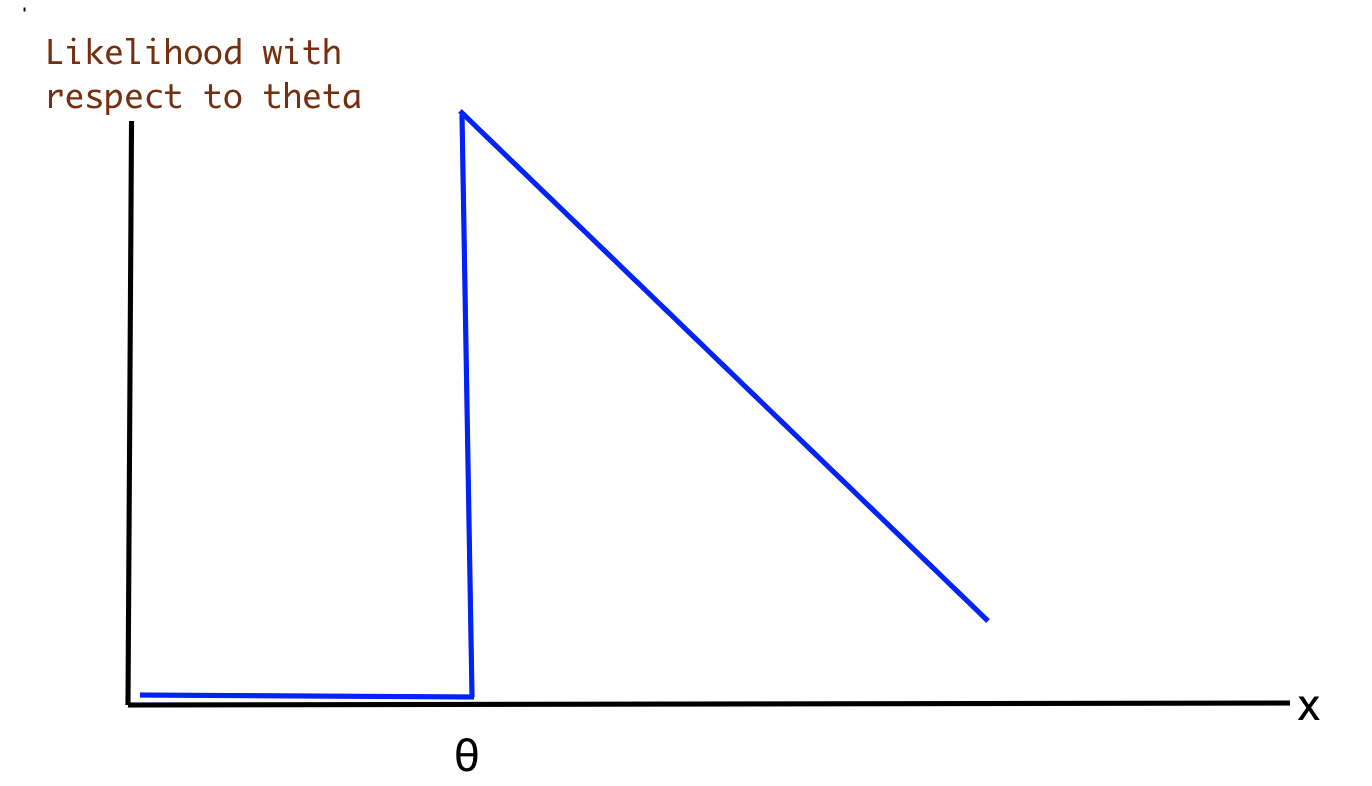
\includegraphics[scale=0.4]{picture_3a.png}
\end{center}

Substitute into equation $3$ to get the estimator for $\lambda$

\[\hat{\lambda} = \frac{n}{\sum{x_i} + n \cdot \text{min}(x_i)} \]

\vspace{3cm}

\subsection*{b)}

\[
  \hat{\theta} = \text{min}(x_i) = 0.64
\]

\[
  \hat{\lambda} 
  = \frac{n}{\sum{x_i} + n \cdot \text{min}(x_i)}
  = \frac{10}{55.8 + 10 \times 0.64} 
  = 0.161
\]

\clearpage

\section*{problem 4}

\textit{Exercise 4 a, d, e on page 390.}

\[ \left(\bar{X} - z_{\alpha/2} \cdot \frac{\sigma}{\sqrt{n}} \hspace{2mm}, \hspace{2mm} \bar{X} + z_{\alpha/2} \cdot \frac{\sigma}{\sqrt{n}} \right)\]

\subsection*{a)}

\[z_{.95/2} = \Phi((1 - .95)/2) = 1.96 \]

\[ \left(58.3- 1.96 \cdot \frac{3.0}{\sqrt{25}} \hspace{2mm}, \hspace{2mm} 58.3 + 1.96 \cdot \frac{3.0}{\sqrt{25}} \right)\]

\[ (57.1, 59.5) \]


\subsection*{d)}

\[ z_{.82/2} = \Phi((1 - .82)/2) = 1.34 \]

\[ \left(58.3- 1.34 \cdot \frac{3.0}{\sqrt{100}} \hspace{2mm}, \hspace{2mm} 58.3 + 1.34 \cdot \frac{3.0}{\sqrt{100}} \right)\]

\[ (57.9, 58.7) \]

\subsection*{e)}

The sample size would need to be 240.

\[n = \left(2 z_{\alpha/2} \cdot \frac{\sigma}{w}\right)^2\]

\[ z_{.99/2} = \Phi((1 - .99)/2) = 1.34 = 2.58 \]

\[n = \left(2 \times 2.58 \times \frac{3.0}{1.0} \right)^2 = 239.6 \]
\end{document}










